% format the chapter/section details
\chapter{Introduction}
\label{chap:intro}

% contained in this file are examples for inserting figures, tables, and equations as well as in text citations
% % figure example 
% \begin{figure}[h!]
%     \centering % center the graphic in the text
%     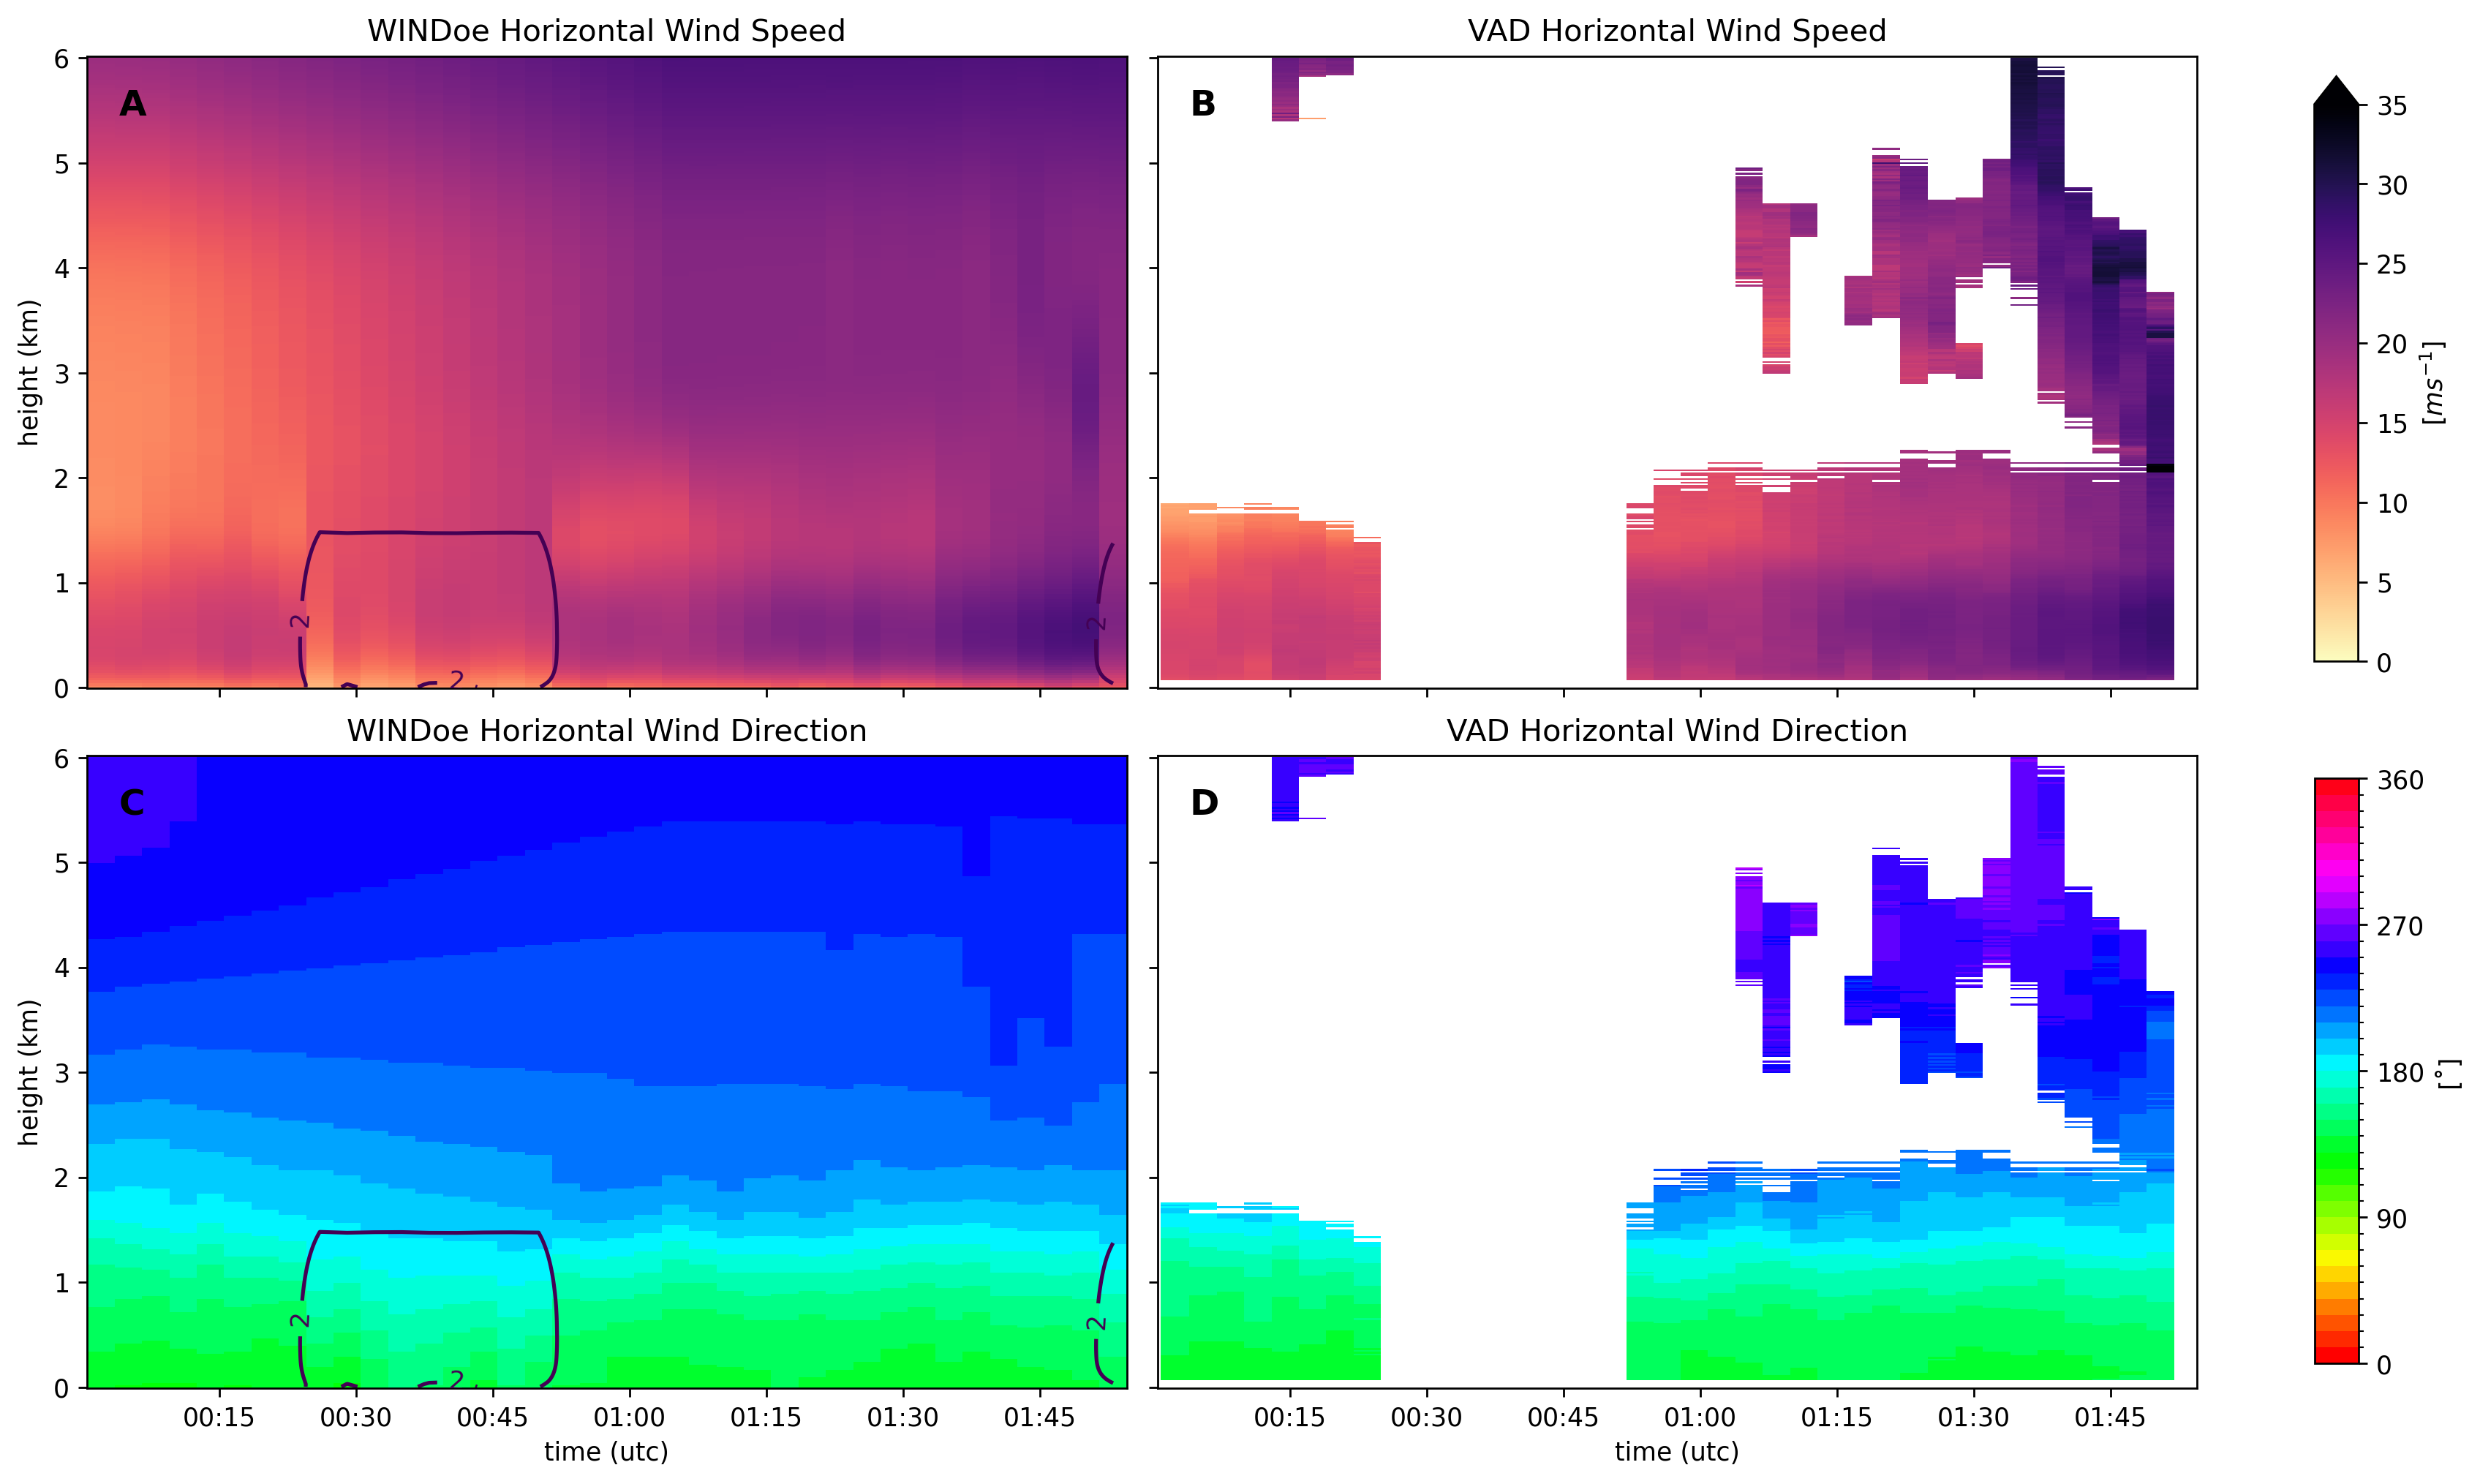
\includegraphics[width=0.7\textwidth]{figures/example.png} % include the figure
%     \caption{some caption} % add a caption
%     \label{fig:some_fig} % label the figure for referencing in the paper
% \end{figure}

% % equation example 
% \begin{equation}
%     \omega_h = (\frac{dw}{dy} - \frac{dv}{dz}, \frac{du}{dz} - \frac{dw}{dx}) % add equation
%     \label{eq:some_eq} % label equation for referencing in paper
% \end{equation}

% % table example
% \begin{table}[h!]
%     \centering % center the table in the text
%     \begin{tabular}{c|c|c} % begin the table with the text orientation of the text in table cells
%         \textbf{variable} & \textbf{variable 2} & \textbf{variable 3} \\\hline % headers
%         test & test & test\\ % values (this is one row)
%         test & test & test\\ % values (this is one row)
%         test & test & test\\ % values (this is one row)
%     \end{tabular}
%     \caption{some caption} % add a caption
%     \label{tab:some_table} % label table for referencing in paper
% \end{table}

% % in text citation example 
% when using this template, please use /citep{} for in text citations (e.g. \citep{smith2020}) and \cite{} for in 
% text citations that are part of the sentence (e.g. \cite{smith2020} found that...)

% insert your text below the line
%-------------------------------------------
A better understanding of supercell thunderstorms and their hazards is critical towards saving a disproportionate number of lives lost compared to other weather-related events \citep{brotzge2013tornado}. Efforts continue in both modeling and observational research to decipher differences between various supercell environments and the downstream hazards associated with storms within them \cite[e.g.,][]{nowotarski2013classifying, parker2014composite, coffer2020near, coniglio2020insights}. Of note, predicting tornadic versus non-tornadic supercells has been particularly difficult \citep{brooks2018long}. These difficulties highlight the importance of storm environment research and developing a better understanding of storm environment variability.

\section{Supercell Thunderstorms}
The term 'supercell' is used to describe a thunderstorm with a rotating updraft, or mesocyclone \citep{browning1962sup}. An early distinction found between supercells and ordinary thunderstorms was their movement separate from the mean wind. \cite{browning1964airflow} created a formal model of the now coined, 'right moving supercell'. As time and research progressed, a supercell was used to describe an anti-cyclonically rotating storm moving to the left or a cyclonically rotating storm moving right of the mean wind. In this study, only right-moving supercells are analyzed. Schematics for these storms were developed by \cite{lemon1979severe} who posed a two dimensional view of supercell structure and it's governing features (Fig. \ref{fig:sup2d}) as well as an evolutionary diagram of the supercell and its associated updraft and downdraft evolution (Fig. \ref{fig:supevolution}). 

\begin{figure}[h!]
    \centering
    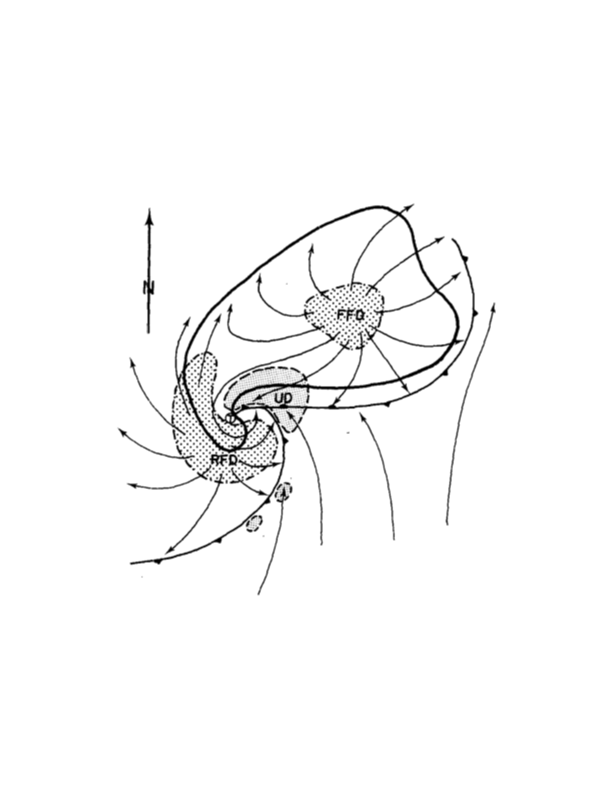
\includegraphics[width=1\textwidth]{figures/supercell_2d.png}
    \caption{One of the first two dimensional views of a supercell and its primary regions. Regions include the forward and rear flank downdraft (FFD/RFD), updraft (UD), and a generalized flow pattern. Figure from \cite{lemon1979severe}. Their figure 7.}
    \label{fig:sup2d}
\end{figure}

\begin{figure}[h!]
    \centering
    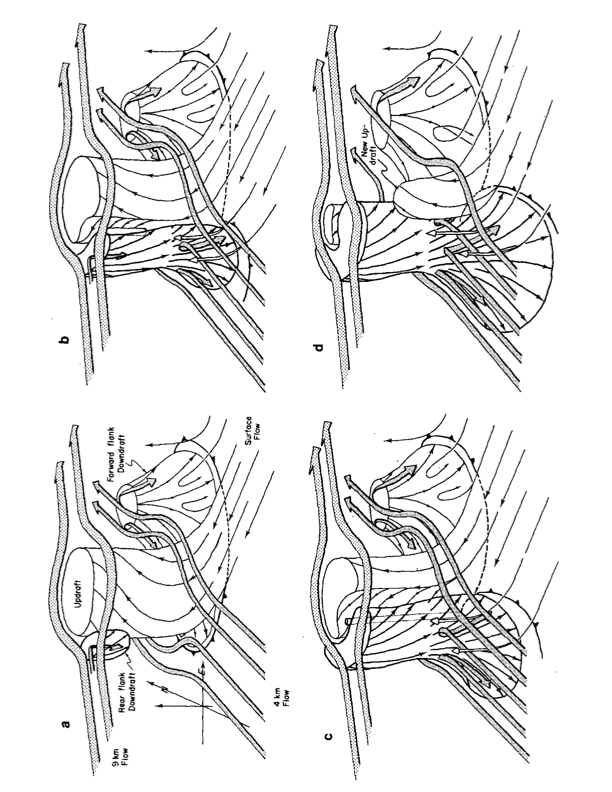
\includegraphics[width=0.75\textwidth, angle = 270]{figures/supercell_evolution.png}
    \caption{Updraft and downdraft evolution during the lifetime of a supercell thunderstorm including mid and upper level flow patters and previously identified storm features. Figure from \cite{lemon1979severe}. Their figure 9.}
    \label{fig:supevolution}
\end{figure}
